\documentclass{article}
\usepackage[margin=0.75in]{geometry}
\usepackage{enumitem}
\usepackage{setspace}
\usepackage{amsmath}
\usepackage{amssymb}
\usepackage{physics}
\usepackage{relsize}
\usepackage{graphicx}
\usepackage{multicol}

\title{CS 143 Final}
\date{3/13/2021}
\author{Jiaping Zeng}

\begin{document}
\setstretch{1.35}

\begin{enumerate}
      \item It is not BCNF; We can first move $F\rightarrow C$ to its own table, i.e. $R_1(A,B,D,E,F)$ and $R_2(F,C)$. Then we decompose $R_1$ into $R_3(A,B,D,E)$ and $R_4(B,D,F)$ since $BD\rightarrow F$. Therefore the final set of tables is $R_2(F,C),R_3(A,B,D,E),R_4(B,D,F)$.
      \item
            \begin{enumerate}
                  \item We have $\{C,D,E,F,G,H\}$ that has no dependencies, which makes $2^6=64$ closed sets. Then since a closed set with $B$ must also have $C,D$ in it, we have another $2^4=16$ sets (since $\{E,F,G,H\}$ makes 16 combinations). Then we can add $A$ to those $16$ sets to make 16 more. Therefore we have $64+16+16=96$ closed sets in total.
                  \item Any subset that implies $A\rightarrow B$ must contain either or both $\{A\rightarrow B\}$ and $\{A\rightarrow C,C\rightarrow B\}$. Then we can make 8 combinations that does not logically imply $A\rightarrow B$ with $\{B\rightarrow A,C\rightarrow A,B\rightarrow C\}$, then another 8 from those combinations with $A\rightarrow C$ added (and not $C\rightarrow B$), simiarly, we have another 8 with $C\rightarrow B$ added. Therefore the number of subsets that implies $A\rightarrow B$ is $64-8-8-8=40$.
            \end{enumerate}
      \item
            \begin{itemize}
                  \item [I:] CBAD: guaranteed to empty; Table C can be deleted first since no other table depends on it. Then B can be deleted since although D(z1) depends on B(x) it has ON DELETE SET NULL specified and it is nullable. A can now be deleted since D(z2) is also nullable.
                  \item [II:] CDAB: not guaranteed to empty; A is deleted before B so B(x) will be set NULL but it is a PRIMARY KEY and cannot be set NULL.
                  \item [III:] BCDA: guaranteed to empty; B is deleted first and D(z1) is set NULL, C is then deleted since nothing references it. D can then be deleted since A is not dependent on it.
            \end{itemize}
      \item
            \begin{enumerate}
                  \item $ $
                        \begin{center}
                              \begin{tabular}{|c|c|c|c|}
                                    \hline
                                              & INSERT                      & DELETE & UPDATE                        \\
                                    \hline
                                    Executive & YES (insert high pay)       & NO     & YES (raise pay past 10 times) \\
                                    \hline
                                    Employee  & YES (insert new lowest pay) & NO     & YES (lower lowest pay)        \\
                                    \hline
                              \end{tabular}
                        \end{center}
                  \item CHECK (salary $<=$ (SELECT 10*MIN(salary) FROM Employee WHERE division = div\_in\_charge))
            \end{enumerate}
      \item SELECT publisher, SUM(price) as a1\\FROM Books\\WHERE birthYear$>$1950\\GROUP BY publisher\\HAVING SUM(price)$>$10000;
      \item
            \begin{enumerate}
                  \item missing the average rotational latency - $r$, since the head might not start at the beginning of the file;\\Access time = seek time + rotational delay + transfer rate = 10ms + r + 1/(6000/60) = 10ms + r + 10ms = r + 20ms.
                  \item 9804; $\lfloor\dfrac{4096\text{ bytes/block}}{40\text{ bytes/tuple}}\rfloor=102\text{ tuples/block}$, $\lceil\dfrac{1000000\text{ tuples/table}}{102\text{ tuples/block}}\rceil=9804\text{ blocks/table}$.
                  \item Each block is 4096 bytes so each one can fit 255 longs and 256 pointers. So we have $\lceil\dfrac{1000000}{255}\rceil=3922$ leaf nodes, $\lceil\dfrac{3922}{256}\rceil=15$ level 2 nodes, and $\lceil\dfrac{15}{256}\rceil=1$ root node. Therefore we need at least $3922+15+1=3938$ ndoes.
                  \item 3 IOs; 2 IOs from root to level 3, 1 IO from level 3 to data.
            \end{enumerate}
      \item
            \begin{enumerate}
                  \item  $ $
                        \begin{center}
                              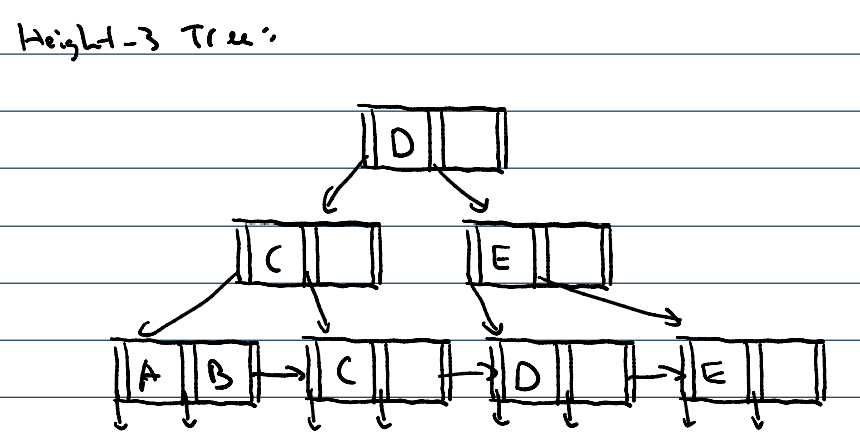
\includegraphics{7a.png}
                        \end{center}
                  \item $ $
                        \begin{center}
                              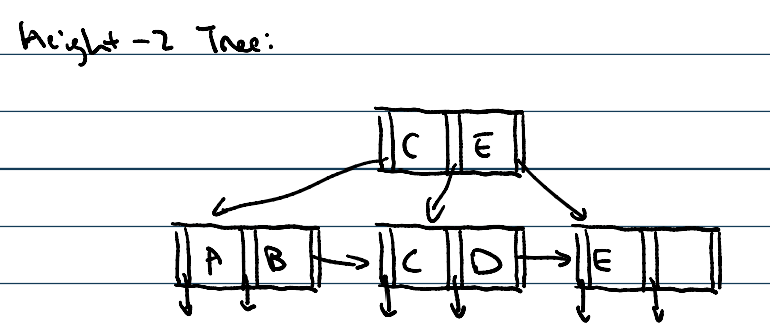
\includegraphics{7b.png}
                        \end{center}
            \end{enumerate}
      \item
            \begin{enumerate}
                  \item $ $
                        \begin{center}
                              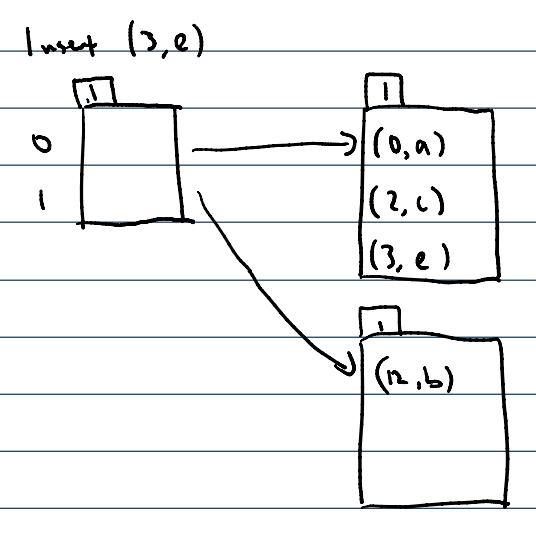
\includegraphics{8a.png}
                        \end{center}
                  \item $ $
                        \begin{center}
                              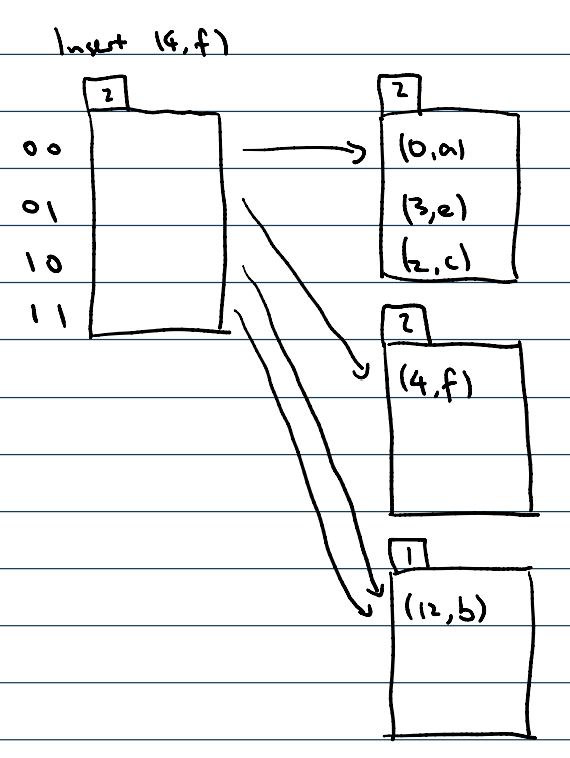
\includegraphics{8b.png}
                        \end{center}
            \end{enumerate}
\end{enumerate}

\end{document}